%*******************************************************************************
% Example chapter file for books, Copyright A K Peters, Ltd.
%*******************************************************************************
\chapter{The Title of Your Chapter}{John Smith and Jane Doe}
 \label{Your-chapter}

\section{Introduction}

This template is for your use in writing your chapter. We have set up section headings, labels, and other elements for you to use as you write. When we receive your article, we will compile it into a book that includes all the other contributions by other authors. Consequently, it's important for you to follow the guidelines here and not introduce variations that may make your article incompatible with others in the book.

The following guidelines will help ensure that your article is consistent with the other chapters in the book, both in terms of the formatting (use the .tex, .bst, and .sty files we have provided) and in terms of organization (all chapters in the book should have a similar style, including beginning with an introduction, using headings in the body of the chapter, and ending with a conclusion and a bibliography).

The structure of this template is designed for you to be able to cut out our words and commands and replace them with your own. It also includes instructions about writing your chapter.

For example, every chapter should begin with an introduction. Please leave the heading above as it is and add text here that introduces readers to what your chapter will be about. Tell readers what the topic of your chapter is, why it is important, and what things you will cover in the chapter.

\section{Your Level-One Section Heading}\label{YourName:SectionLabel}

After the introduction, you may begin however you think is best. One option is to begin by giving readers the context for your topic. It may be helpful to provide the historical underpinnings or theoretical background for your topic. Throughout your chapter, any time you introduce a new \textit{keyword}, set it in italics, as we did in this sentence.

You should also include index entries in your chapter. This is an index entry.\textbackslash index\{index\} An index entry with a subentry looks like this: \textbackslash index\{entry!subentry\}. For an index entry that spans multiple pages, type \textbackslash index\{entry\textbar(\} where you want the entry to start. Type \textbackslash index\{entry\textbar)\} where you want it to end. There are index entries throughout this document that you can see for more examples. Keywords are good place to start in creating your index.

As necessary, divide\index{organization} your chapter into sections with appropriate headings. Section titles should use title capitalization (capitalize the first and last words and everything except articles, prepositions, and conjunctions; capitalize the second word in a hyphenated term, e.g., Real-Time Rendering). These headings should not end in a period.\index{punctuation}

\subsection{Your Level-Two Section Heading}\label{YourName:SubsectionLabel}
If you need further divisions, you can include level-two headings to divide the text. Like level-one headings, these headings should have title-style capitalization.\index{organization}

While it's not necessary to cross-reference parts of your chapter, you can refer to other sections and subsections of your chapter if you create a label for the section.\index{reference} For example, we have made a label for Section~\ref{YourName:SectionLabel}. Throughout your chapter, as you create labels (e.g., for sections, figures, listings, equations, etc.), please include your surname as part of the label so that once we combine all the chapters from all the various authors, we do not have redundant labels. Any time you reference something, please use a \texttt{ref} command rather than a hard-coded number.

As you set up your organization, do not use a lower-level section heading without a corresponding higher-level section heading. For example, do not jump from a section to a subsubsection without having a subsection in between.

\subsubsection{Level-three section heading.}\label{YourName:SubsubectionLabel}
It is not common to need a third level of heading, but you may use level-three headings if you need them. In these headings, capitalize only the first word and any proper nouns, and end the heading with a period.\index{punctuation}

These headings run in with the first paragraph of the section and are not numbered, which means you cannot
refer to such sections by number.\index{reference}

Another option for breaking up the text is to include bulleted or numbered lists.
\begin{itemize}
 \item Unnumbered lists are structured like this.
 \item They can have as many items as you need.
\end{itemize}

\begin{enumerate}
 \item Numbered lists are structured like this.
 \item You should only use numbers if the order of the things you are listing matters.
\end{enumerate}


\section{Your Level-One Section Heading}

This is the main part of your paper, where you provide the details of your topic. There are many ways to share this information.

\subsection{Equations}
You can include mathematical expressions as needed. If you are going to refer back to equations, you should set them up as numbered equations, as we have done in Equation~\eqref{Smith-slope-int}.\index{reference} When you refer to the equation, please use \texttt{eqref}, which will produce parentheses around the equation number. This is an example of a numbered equation:
\begin{equation}\label{Smith-slope-int}
y=mx+b.
\end{equation}
If you are going to talk about an equation only in the paragraph where it appears, and will not refer back to it, set it up as an unnumbered equation, like this one:
$$
y = \frac{-b \pm \sqrt{b^2 - 4ac}}{2a}.
$$

\subsection{Code}
You may also want to provide algorithms, such as snippets of code or pseudocode. If you use short bits of code, put them in like this:
\begin{verbatim}
out vec3 fragmentColor;
\end{verbatim}
You may also set words in the regular paragraph in a \texttt{code font}.

If you choose to use syntax highlighting, please specify the language you are using, as is done in the preamble (``language=C'') of Listing~\ref{YourName:listing1}.

If you are including longer listings, set them up like Listing~\ref{YourName:listing1}. Longer listings like this should always include a caption. They should also be referenced in the text, as we did in the first sentence of this paragraph, so that readers can easily identify which part of the text is associated with the listing, and vice versa.\index{reference}

\begin{lstlisting}[language=GLSL,float={htb},caption={Your caption.},label={YourName:listing1}]
in vec3 worldPosition;
in vec3 positionToLight;
out vec3 fragmentColor;

void main()
{
  // Calculate diffuse lighting
  vec3 toLight = normalize(positionToLight);
  vec3 normal = normalize(worldPosition);
  float diffuse = max(dot(toLight, normal), 0.0);
  fragmentColor = vec3(diffuse, diffuse, diffuse);
}
\end{lstlisting}

In general, use references (for example, see Listing~\ref{YourName:listing1}) and avoid phrases such as ``in the following algorithm'' or ``in the figure below.'' In the final typesetting, long listings, figures, and tables may end up being before or after where they are mentioned in the text.\index{reference!justification}

Please note that, except in rare cases, code should not run on for many pages. If it's needed, such code could be included in the book's supplemental online material.

\subsection{Tables}
Tables are also a good complement to text (see Table~\ref{YourName:table1}). Like figures and long listings, tables should be referenced in the text and have a caption.\index{reference}
\begin{table}[htb]\centering
\begin{tabular}{|c|c|c|}
\hline%
\small{Parameters} & \small{Result A} & \small{Result B}\\
\hline%
\small{X} & \small{1} & \small{2}\\
\hline%
\small{Y} & \small{3} & \small{4} \\
\hline%
\end{tabular}
 \caption{Your caption.}
 \label{YourName:table1}
\end{table}

\subsection{Figures}
You may want to include figures that complement what you are explaining. These may include diagrams, models, screenshots, or other figures you create.\index{figure}

Because your article will be gathered with many others into a single book, you'll need to use a file format that is compatible with all the other authors' files. Consequently, you may use .jpg, .png, and .pdf files but \emph{not} .eps files.
For any figure you include, be sure to mention it in the text.\index{reference}
Please put figures near where they are mentioned in the text, but do not worry about sizing or exactly placing figures, as all of this will be adjusted in the final typesetting.

Don't forget to send us all figure files in addition to your \LaTeX files at the time you submit your chapter.\index{figure}

\subsubsection{Permissions.}
If the rights to a figure are owned by someone else, as soon as possible please obtain permission to use the figure. If needed, we can provide a template of a permission form that you can use to obtain permission from the
copyright holder. Once you have received permission, please send a copy of that permission release to us for our records. To credit the copyright holder of an image, include a statement in brackets at the end of the caption, as we have done in Figure~\ref{YourName:fig1}.\index{figure!permission}

\begin{figure}[htb]\centering

\includegraphics[width=.2\textwidth]{akp}
\caption{Your caption. [Image courtesy Permission Grantor]}\index{figure!permission}
\label{YourName:fig1}
\end{figure}

\subsubsection{Color.}
All figures must be supplied in either grayscale or, if color will be used in the book, CMYK is preferred. RGB files will be converted to CMYK before printing. Figure~\ref{YourName:fig2} is a color figure.
If you are working with images in RGB color format, such as screenshots, be aware that colors generally shift when converted to CMYK. Many bright, vibrant colors you can create in RGB just cannot be matched in CMYK. If you are concerned about keeping vivid colors, avoid using colors that are close to pure red, green, or blue as they will always look desaturated; cyans, yellows, and dark colors convert more easily. Also avoid very dark images, as details of these will likely not show up in printing.\index{figure!color}

\begin{figure}[htb]\centering
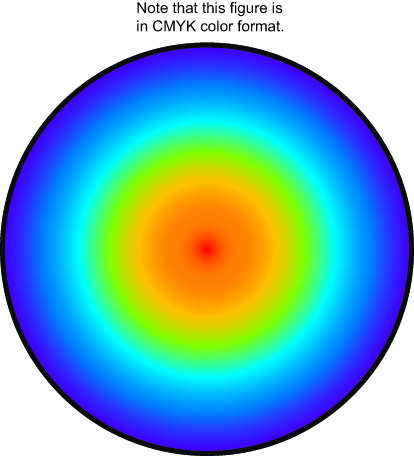
\includegraphics[width=.55\textwidth]{circle}
\caption{Here is a sample figure.}
\label{YourName:fig2}
\end{figure}

\subsubsection{Resolution.}
For best printing quality, images need to have a resolution of 300 dpi at the full size in which they will appear on the printed page. Images from the internet are often low-resolution, so please check their quality before you choose to include them in your book.

If you are creating images or scanning them yourself, create them at the size they will appear in the printed version of the book.\index{figure!resolution}

\subsubsection{Labels.}
If you add labels to your images, bear in mind that text in the image should be slightly smaller in size than the main text of the book: use Arial, 9 pt.\ font.\index{figure!label} To ensure that labels look consistent in all images, please first size your image to approximately the size it will appear in the book and then add the labels (if you make an image that is 30cm$\times$30cm and then we scale it down to fit in the book, the labels will look tiny).

\section{Your Level-One Section Heading}

After you have given all the details about your topic, you may also consider including an analysis of your topic.
Are there limitations to what you've described? What are the tradeoffs? What are its strengths and weaknesses compared to alternatives?

\section{Conclusion}

Every chapter should end with a conclusion.\index{organization} Please leave the heading name as it is (i.e., ``Conclusion''), and in this paragraph put your concluding remarks. Your conclusion might include a review of what you've covered in the chapter, projections for future possible work, or suggestions for implementing what you have discussed.

Once we receive your chapter, we will ensure that it is copyedited for grammar, punctuation,\index{punctuation} and consistency with other chapters. We will then typeset the chapter, incorporating it into the rest of the book and doing the layout of the entire book. While we ask that you make the quality of your text, figures, and code as good as possible before you submit the chapter, you do not need to make any changes to the format or appearance of the electronic files (e.g., changing the fonts used, altering page dimensions, inserting manual line breaks, putting in spacing commands, etc.), as we will likely override any such adjustments.

The last part of your chapter is the bibliography. You can include a bibliography using the commands below.\index{citation}
For books and proceedings, be sure to include the author, title, publisher, place of publication, year, and article title and pages if applicable. For journal articles include the author, article title, journal title, volume, issue, year, and pages of the article. For websites, include the author, title, webpage title, date of posting or access, and url. The bibliography will include any sources that were referenced in the text, such as  \cite{Gunter09,Smith06,Gomez07,Wang11}.

\bibliographystyle{akpbib}
\bibliography{YourBib}











